\chapter{虚拟化与kvm}
KVM 全称是 基于内核的虚拟机(Kernel-based Virtual Machine),它是Linux 的一个内核模块,该内核模块使得 Linux 变成了一个 Hypervisor:
KVM 是基于虚拟化扩展(Intel VT 或者 AMD-V)的 X86 硬件的开源的 Linux 原生的全虚拟化解决方案。

KVM 中,虚拟机被实现为常规的 Linux 进程,由标准 Linux 调度程序进行调度;
虚机的每个虚拟 CPU 被实现为一个常规的 Linux 线程。这使得 KMV 能够使用 Linux 内核的已有功能。
  但是,KVM 本身不执行任何硬件模拟,需要用户空间程序通过 /dev/kvm 接口设置一个客户机虚拟服务器的地址空间,
  向它提供模拟 I/O,并将它的视频显示映射回宿主的显示屏。目前这个应用程序是 QEMU。
  
\section{虚拟化}
X86操作系统是设计在直接运行在裸硬件设备上的,因此它自动认为完全占有计算机硬件,
X86平台的指令集权限划分为特权模式: Ring0, Ring1, Ring2, Ring3。 操作系统使用Ring0级别;应用程序使用Ring3级别。
驱动程序使用Ring1,Ring2级别。应用程序不能做受控操作,如果需要做,比如要访问硬盘,写文件,那就要通过执行系统调用,执行系统调用的时候CPU的运行级别发生3到0的切换,
并跳转到系统调用对应的内核代码位置执行,内核就为你完成设备访问,完成之后再从0返回3,这个过程也称为用户态的内核态的切换。
X86平台在虚拟化方面的一个难点就是如何将虚拟机越级的指令使用进行隔离。

\begin{figure}[!ht]
    \centering
     \caption{\label{Fig:virtualization-progress} virtualization progress}
    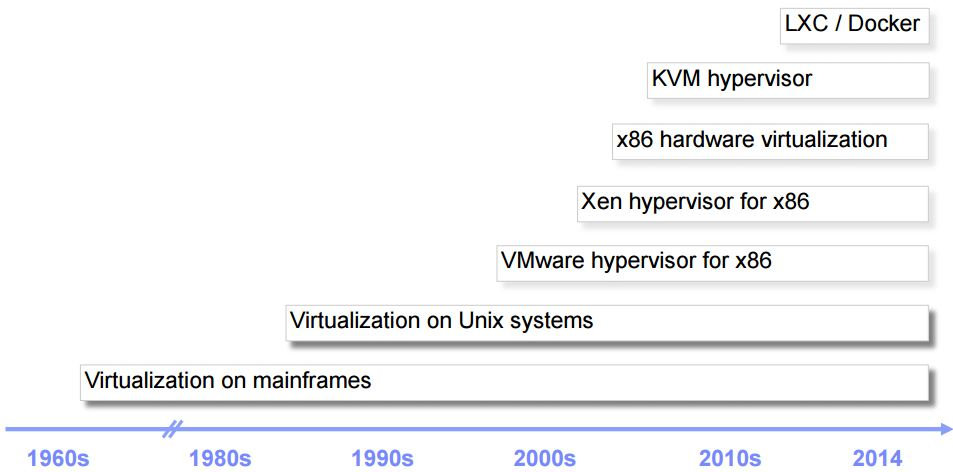
\includegraphics[width=0.8\textwidth]{kvm/virtualization-progress.jpg}
\end{figure}



软件虚拟化、基于二进制翻译的全虚拟化(full Virtualization with Binary Translation):
客户操作系统运行在Ring1,它运行特权指令时,会触发异常(CPU机制,没有权限的指令会触发异常)然后VMM (Virtual Machine Manager)捕获这个异常,在异常里面做翻译,模拟,最后返回到客户操作系统内,客户操作系统认为自己特权指令工作正常,继续运行。但这个性能损耗大。 典型厂商 VMware

\begin{lstlisting}
yum install qemu-kvm qemu-img
yum install virt-install  bridge-utils libvirt
systemctl start libvirtd

qemu-img create -f qcow2 centos-7.1.qcow2 50g
virt-install --name Centos-7.1-x86_64-base  --virt-type kvm \
 --memory 1024 --vcpus 1 \
 --cdrom /data/iso/CentOS-7-x86_64-DVD-1503-01_2.iso \
 --disk path=/base_image/centos-7.1.qcow2,bus=virtio \
 --network network=br0,model=virtio \
 --graphics vnc,listen=0.0.0.0 --noautoconsole
\end{lstlisting}

下面有一个坑, network=br0, 会去找libvirt里network里定义的网络,如果使用bridge,则需要把network=br0 改为bridge=br0既可
如果使用现有qcow2做磁盘,就不需要使用cdrom,直接使用--boot hd既可

创建windows
\begin{lstlisting}
virt-install --name zbddzx_ceshi-05  --ram 8192 --cpus 2 \
 --cdrom=/Data/Base_images/2012R2.iso  \
 --disk path=/opt/zbddzx_ceshi-05.qcow2,bus=virtio  \
 --graphics vnc,listen=0.0.0.0  \
 --network bridge=virbr300,model=virtio \
 --noautoconsole
\end{lstlisting}

guestfish 里面包含很多非常有用的工具,比如virt-copy-in可以把宿主机的文件直接copy进主机
\text{	virt-copy-in /etc/selinux/config  -a /Data/Base_image/CentOS-6.6.qcow2  /etc/selinux/}

安装 KVM 后都会发现网络接口里多了一个叫做 virbr0 的虚拟网络接口,一般情况下,虚拟网络接口virbr0用作nat,以允许虚拟机访问网络服务,但nat一般不用于生产环境。我们可以使用以下方法删除virbr0

1、先使用virsh net-list查看所有的虚拟网络:virsh net-list 
2、卸载与删除virbr0虚拟网络接口 先关闭virsh net-destroy default  再删除virsh net-undefine default

从一个xml文件定义default网络,执行如下命令: \text{virsh net-define /var/lib/libvirt/network/default.xml  }

1、设置virbr0自动启动,执行如下命令:virsh net-start default           

2、自启动 virsh net-autostart default    


